\documentclass[12pt]{article}
\usepackage{arydshln}
\usepackage[hidelinks]{hyperref}
%\renewcommand{\baselinestretch}{1.5}
\usepackage[onehalfspacing]{setspace}
\setlength{\footnotesep}{0cm}
\usepackage[spanish]{babel}
\usepackage[utf8]{inputenc}
\usepackage{mathptmx}
\usepackage{courier}
\usepackage{helvet}
\usepackage[T1]{fontenc}
\usepackage[paper=letterpaper,left=3cm,right=3cm,top=2cm,bottom=3cm]{geometry} 
\usepackage{framed,color}
\usepackage{graphicx}
\definecolor{shadecolor}{rgb}{0.1,0.1,0.1}
\usepackage{tocloft}
\renewcommand{\cftsecleader}{\cftdotfill{\cftdotsep}}
\usepackage{titlesec}
\titleformat{\section}{\singlespacing\normalfont\Large\bfseries\scshape}{\thesection.}{1em}{}
\titleformat{\subsection}{\singlespacing\normalfont\large\bfseries\scshape}{\thesubsection}{1em}{}
\usepackage[table]{xcolor}
\colorlet{tableheadcolor}{lightgray}
\usepackage{parskip}
\setlength{\parindent}{15pt}
\usepackage{multirow}
\usepackage{longtable}
\usepackage{pdfpages}
\setcounter{tocdepth}{1}
\usepackage{float}
\restylefloat{table}

\begin{document}

%\renewcommand{\contentsname}{\begin{center} TABLA DE CONTENIDOS \end{center}}
\renewcommand{\contentsname}{\begin{center}TABLA DE CONTENIDOS\end{center}
\begin{flushleft}{\small Título}\end{flushleft} \vspace{-1cm} \begin{flushright}{\small Página}\end{flushright}}
\renewcommand{\refname}{}

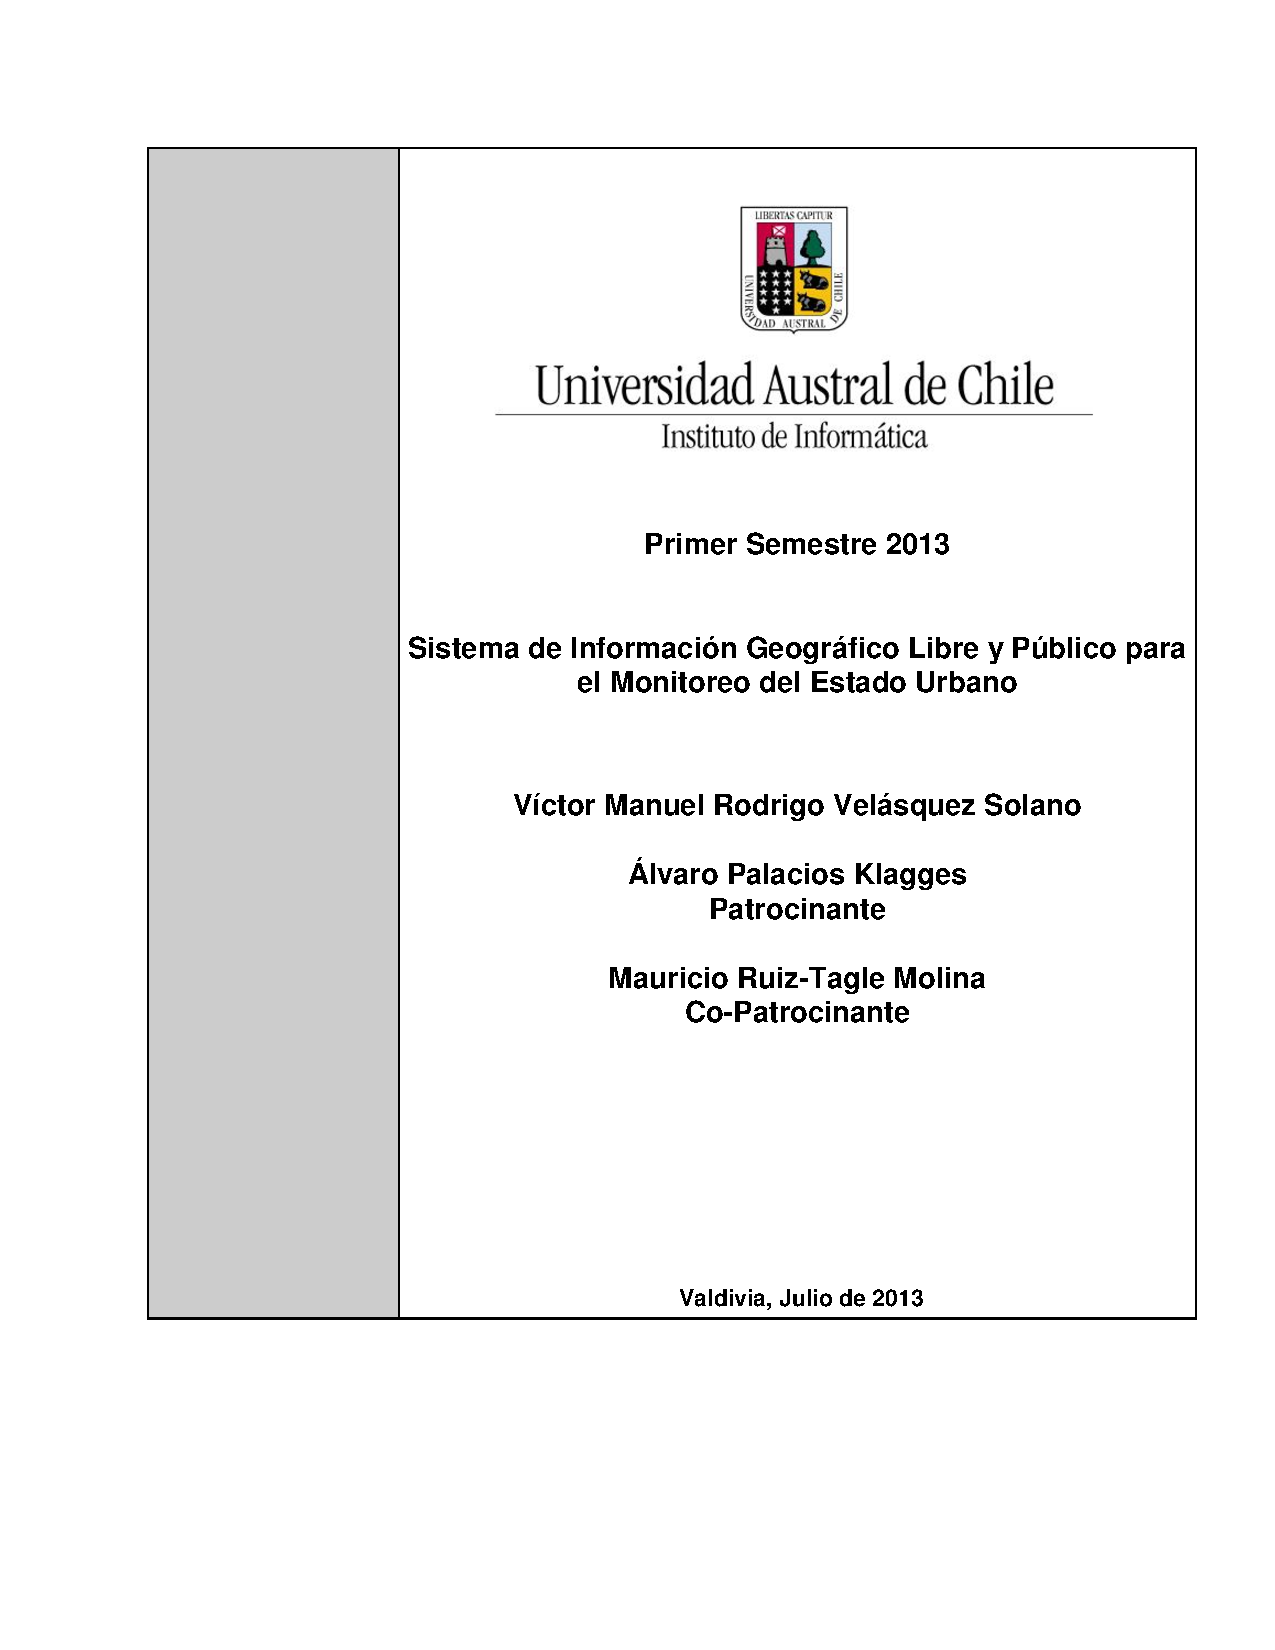
\includepdf[pages={1}]{imagenes/portada.pdf}
\tableofcontents

\newpage
\section{presentación general}
\subsection{título del proyecto}
\begin{table}[h]
	\centering
	\begin{tabular}{|p{\textwidth}|}
    \hline
    \multicolumn{1}{|>{\columncolor{lightgray}}p{\textwidth}|}{Sistema de
      Información Geográfico Libre y Público para el Monitoreo del Estado
      Urbano }
    \\
    \hline
	\end{tabular}
\end{table}

\subsection{dominio}
\begin{table}[!h]
	\centering
	\begin{tabular}{|p{\textwidth}|}
    \hline
      Ciencias de la Computación e Ingeniería de Software
      \\
    \hline
	\end{tabular}
\end{table}


\subsection{disciplina científica y tecnológica}
\begin{table}[!h]
	\begin{tabular}{|p{2cm}|p{12.55cm}|}
    \multicolumn{2}{l}{Código} \\
      \hline
      75 & Ingenería en Computación \\ \hline
  \end{tabular}
\end{table}

\subsection{áreas de aplicación}
\begin{table}[!h]
	\begin{tabular}{|p{2cm}|p{12.55cm}|}
        \multicolumn{2}{l}{Código} \\
        \hline
        167 & Sociología Urbana y Rural \\ \hline
	\end{tabular}
\end{table}

\subsection{duración del proyecto}
\begin{table}[!h]
	\begin{tabular}{|p{1cm}|p{1cm}|l}
        \cline{1-2}
        \cellcolor{lightgray} 0 & \cellcolor{lightgray} 6 & Meses \\
        \cline{1-2}
    \end{tabular}
\end{table}

\newpage
\section{responsables del proyecto}
\subsection{institución principal del proyecto}
\begin{table}[!h]
	\centering
        \begin{tabular}{|p{4.7cm}|p{4.7cm}|p{4.8cm}|}
        \hline
        \multicolumn{2}{|l|}{\textbf{Nombre de la Institución}} &
        \textbf{RUT} \\
        \multicolumn{2}{|l|}{SECPLAN Ilustre Municipalidad de Valdivia}
        & -- \\ \hline
        \multicolumn{2}{|l|}{\textbf{Dirección}} & \textbf{Ciudad} \\
        \multicolumn{2}{|l|}{Independencia \# 445} & Valdivia \\ \hline
        \textbf{Teléfono} & \textbf{Fax} & \textbf{E-mail} \\
        -- & -- & -- \\ \hline
	\end{tabular}
\end{table}

\subsection{patrocinante del proyecto}
\begin{table}[h]
	\centering
	\begin{tabular}{|p{3.4cm}|p{3.4cm}|p{4.4cm}|p{2.4cm}|}
        \hline
        \multicolumn{2}{|l}{\textbf{Nombre Completo}} &
        \multicolumn{2}{|l|}{\textbf{RUT}} \\
        \multicolumn{2}{|l}{Álvaro Palacios Klagges} &
        \multicolumn{2}{|l|}{15.481.574--4} \\ \hline
        \multicolumn{2}{|l}{\textbf{Dirección}} &
        \multicolumn{2}{|l|}{\textbf{Ciudad}} \\
        \multicolumn{2}{|l}{Independencia \# 445} &
        \multicolumn{2}{|l|}{Valdivia} \\ \hline
        \multicolumn{4}{|l|}{\textbf{Cargo Actual}}\\
        \multicolumn{4}{|l|}{Cargo\_Álvaro}\\ \hline
        \textbf{Teléfono} & \textbf{Fax} & \textbf{E-mail} & \textbf{Casilla} \\
        -- & -- & apalacios@munivaldivia.cl & -- \\ \hline
	\end{tabular}
\end{table}
\subsection{datos del estudiante}
\begin{table}[h]
	\centering
	\begin{tabular}{|p{3.4cm}|p{3.4cm}|p{4.0cm}|p{2.8cm}|}
        \hline
        \multicolumn{2}{|l|}{\textbf{Nombre Completo}} &
        \multicolumn{2}{l|}{\textbf{RUT}} \\
        \multicolumn{2}{|l|}{Víctor Manuel Rodrigo Velásquez Solano} & 
        \multicolumn{2}{l|}{17.066.860 -- k} \\ \hline
        \multicolumn{2}{|l|}{\textbf{Dirección}} & 
        \multicolumn{2}{l|}{\textbf{Ciudad}} \\
        \multicolumn{2}{|l|}{Pasaje José Ramirez, Departamento 1252-C} & 
        \multicolumn{2}{l|}{Valdivia} \\ \hline
        \textbf{Teléfono} & \textbf{Fax} & \textbf{E-mail} &
        \textbf{Casilla} \\
        (+56) 9 9695 5466 & -- & victor.mrvs@gmail.com & -- \\ \hline
	\end{tabular}
\end{table}

\newpage
\section{resumen del proyecto}
\noindent \textbf{Título:}
Sistema de Información Geográfico Libre y Público para el Monitoreo del Estado
Urbano.\\


\noindent \textbf{Resumen:} 
	Al momento de postular a proyectos de urbanismo se hace necesario de
	disponer de información actualizada y de rápido acceso que describa el
	espacio urbano de acuerdo a las especificaciones requeridas por el
	gobierno. Esta información, si existe, es susceptible a problemas como:
	la obsolescencia, no estandarización de los datos, dispersión e
	inaccesibilidad. Además, corresponden a una visión subjetiva parcial de
	la única persona que capturó los datos. En caso de que esta información
	no se encuentre disponible, se recurre a la captura de estos datos,
	proceso que ralentiza los proyectos de mejoramiento urbano al disponer
	recurso humano y monetario en esta recopilación de información.

	Este proyecto implementará una plataforma web colaborativa y escalable
	que permitirá el monitoreo del estado de \emph{elementos espaciales} de
	un espacio urbano. Que sea colaborativa se refiere a la capacidad que
	tienen múltiples usuarios de adjuntar información a la plataforma y la
	capacidad de interacción entre los mismos. Con escalable, desde la
	mirada del usuario,  se refiere a la capacidad de adaptarse a los
	cambios exigidos por el gobierno en materia urbanística; en tanto, en el
	sentido técnico, se refiere a la capacidad de adaptarse a un incremento de
	usuarios e información durante la vida útil de la plataforma, este
	elemento es muy importante a la hora de elegir las herramientas de
	software que se utilizarán.

	La plataforma web colaborativa y escalable, acorde a las necesidades
	contemporáneas, será de fácil utilización y acceso para el usuario y,
	mediante la utilización de Software Libre, permitirá la confluencia de
	información proveniente de distintas fuentes que describen el estado
	actual del espacio urbano acorde a métricas previamente establecidas y
	definidas. La información que se generará en esta plataforma será de
	dominio público, por tanto, de libre utilización por distintos
	organismos e instituciones, ya sean públicas o privadas, con la sola
	restricción de que la información extraída deberá permanecer libre.

  Con esta plataforma se conseguirá un aumento significativo en la productividad de los equipos de
  planificación de proyectos de renovación urbana, al obtener información de manera rápida y
  confiable sobre el espacio urbano de su estudio. Además, es importante para los habitantes poder
  conocer su entorno y como sus vecinos entienden su espacio en común, a través de la plataforma web
  podrán delimitar su barrio y comprenderán su espacio, traduciéndose en un apropiamiento del mismo.

\newpage
\section{objetivos generales y específicos}
\subsection{objetivo general}
Se implementará una plataforma web colaborativa y escalable que permitirá el
monitoreo y actualización del estado de ``elementos espaciales'' definidos en
la documentación de requisitos de postulación a proyectos de mejora urbana. La
plataforma utilizará tecnologías libres en su diseño e implementación, y la
información que generará será de acceso público y de libre utilización. Además,
deberá presentar la flexibilidad suficiente para adaptarse a los cambios del
entorno en cuanto a la legislación y cambios físicos del área urbana.

\subsection{objetivos específicos}
\begin{itemize}

	\item Estudios de conceptos clave de urbanismo y una breve introducción a los procesos de
    urbanización América Latina; estudios generales sobre  
    los Sistemas de Información Geográficos.

	\item Estudio del desarrollo del urbanismo en Chile, sus aspectos técnicos y legales.
    Profundización de los estudios de los Sistemas de Información Geográficos especificando
    herramientas de software presentes.

	\item Definición de los requisitos de usuario y
        requisitos de software, estableciendo como restricciones las
        herramientas de software evaluadas en el estudio anterior.

	\item Desarrollar e implementar la plataforma
        web colaborativa y escalable utilizando un marco de trabajo
        DSDM, basado en un proceso iterativo e incremental.

	\item Desarrollar pruebas y análisis de la
        implementación de la plataforma web, verificando la satisfacción
        de requisitos y pruebas de usabilidad.
\end{itemize}

\newpage
\section{descripción del proyecto}

\subsection{introducción}

La urbanización es un fenómeno social que surge a medida que las sociedades se
van haciendo más complejas, el trabajo en las sociedades urbanas ya no solamente
se preocupa de transformar directamente el entorno, sino también de transformar
los elementos pertenecientes a la super-estructura social. Por consiguiente, el
foco del trabajo ya no está enfocado netamente en la construcción de viviendas
ni elementos relativos, razón por la cual la sociedad define estándares y
prototipos en torno a la construcción de elementos necesarios para la vivienda y
el desarrollo de la misma sociedad. Entre estos elementos encontramos desde la
tipología de la vivienda hasta la distancia entre los paraderos de locomoción
colectiva. Un barrio no es unicamente un conjunto de casas, debe tener una
funcionalidad con sus habitantes. 

``Es claro que la ciudad es la manifestación en el espacio de una
sociedad y como tal crece, se desarrolla y a veces también muere.
Las formas que va tomando el crecimiento urbano son la expresión de las interacciones entre las
fuerzas, políticas, económicas y sociales''.\cite{Mar13}

La transformación del entorno responde a necesidades sociales y la
materialización de estas preocupaciones es una consecuencia política, por lo que
se hace necesario que cada sector que conforma la sociedad tenga la capacidad de
articularse para poder decidir como transformar su entorno. Sin embargo, la
definición del espacio urbano es un aspecto transversal que no puede aplicarse a
un grupo reducido, es de importancia para todos los habitantes del espacio, con la
amplitud que aquello indica. 

Estos sistemas complejos que se conforman en los barrios, unidades vecinales,
juntas de vecinos y otros, requieren de una plataforma común que permita
unificar dos elementos: (1) conocer el entorno en el que se desarrollan y (2) generar
propuestas en esta materia, es decir, una plataforma que permita centralizar la
información y en base a ella permita generar una propuesta.\cite{Pav08}

Actualmente en Chile, el espacio urbano se ve afectado por varios problemas. Las
desigualdades económicas se hacen eco visual en los barrios, la cantidad de
focos de basura, el mal estado de las áreas verdes, calles no pavimentadas, mal
estado del pavimento, abundancia de sectores no habilitados, por mencionar
algunos de los problemas. 
El cambio de este estado depende de dos factores: (1)
que los habitantes tengan clasas
sus posibilidades de transformación y sus deberes con su entorno utilizando la
poca información disponible y de fácil acceso y (2) la
ausencia de un espacio donde se almacenan los datos necesarios para obtener una visión
global y precisa del estado del barrio, permitiendo corregir los problemas
existentes y predecir futuros problemas.\cite{L01}

En este proyecto de título se implementará una plataforma web colaborativa y
escalable que permitirá centralizar la información, relativa al espacio urbano.
Esta información es relativa a lo que aparece en el artículo 1.1.2 de la
OGUC\footnote{OGUC: Ordenanza General de Urbanismo y Construcciones} y a la
simbología utilizada para el concurso \emph{Desarrollo de Barrios} del
MINVU\footnote{Ministerio de Vivienda y Urbanismo de Chile}. 
Facilitará los procesos de postulación a proyectos de mejoramiento
urbano que se presentan como parte de políticas públicas.

La plataforma será web para asegurar acceso universal a la misma. Además será
una plataforma libre en su concepción, uso y desarrollo, es decir, será
trabajada utilizando software libre, el código generado será software libre y la
información generada en la misma será de carácter libre.

La plataforma web debe ser colaborativa dado que la mejor forma de describir el
espacio es por quienes lo utilizan, son los mismos vecinos los que conocen el
estado de sus calles, los focos de delincuencia, los espacios no utilizados, el
estado de las áreas verdes. Por tanto, permitirá el ingreso de información por
distintas organizaciones institucionalizadas, como juntas de vecinos y otros.

La plataforma web será escalable puesto que, al ser eminentemente social, debe
adaptarse a los cambios que ello implica. Debe adaptarse al aumento de la
demanda de la plataforma y al aumento de la información almacenada en la misma.
Además, deberá tener la capacidad de adaptarse a los cambios requeridos por el
gobierno en materias de obras públicas de urbanismo, como los elementos
necesarios a considerar, las escalas métricas, las tecnologías utilizadas.

El efecto esperado con esta plataforma es justamente el
empoderamiento y apropiamiento de los habitantes con respecto a su espacio, como
poder delimitar su barrio, y dar
pié a proyectos de regeneración y renovación urbana.
Además, busca ser una herramienta eficaz que entregue información rápida,
actualizada y verídica sobre la delimitación de un espacio urbano a entidades
que trabajen en proyectos relativos a recuperación de barrios u otros proyectos
afines.

\subsection{nivel actual}
En el plano nacional de administración pública, la poca utilización de bases de datos
relacionales y espaciales, junto a la descentralización de la información, genera inconvenientes a la
hora de estudiar la situación actual del espacio urbano, dado que el acceso a
los datos no asegura que estos estén actualizados. En los municipios, es común que no se
utilicen recursos informáticos e impriman un mapa de las Unidades Vecinales para trabajar a
mano. Todavía se usan hojas de cálculo para almacenar la
información. Son pocas áreas las que se han aventurado a utilizar Sistemas de
Información Geográficos, como el software \emph{ArcGIS}, de ESRI\footnote{ESRI:
Las siglas corresponden a \emph{Environmental Systems Research Institute}}, pero
además de ser software propietario y privativo, su uso corresponde a la
iniciativa propia de encargados en departamentos específicos y no por ordenanza
municipal, tal es el caso de las comunas de San Antonio y Maipu en Santiago.

A nivel universitario, los Sistemas de Información Geográficos (GIS, por sus
siglas en inglés) son enseñados principalmente en
carreras como Geografía y Arquitectura, aunque en esta última es sólo en
talleres de urbanismo. Al menos en la Universidad Austral
de Chile, a través del Laboratorio de Urbanismo, se enseña a utilizar
herramientas GIS como \emph{ArcGIS} y \emph{Space syntax}.

Por otro lado, en el escenario internacional, vemos un avance en cuanto a
sistemas de información geográficos y su utilización en el sector público. Se
conoce de distintos programas aislados, pero es difícil obtener una visión real
del impacto y despliegue ``oficial'' que está teniendo el uso de GIS libres en la
administración pública, principalmente porque el software libre recién está
difundiéndose en las administraciones públicas del mundo como es el caso de
Alemania, Argentina, Brasil, Cuba, Chile, China, Ecuador, España, Francia,
 México, República Dominicana y Venezuela; entre otros.
 OSGeo (\textit{Open
 Source Geospatial Foundation}) mantiene una amplia
lista con la contribución de
diversos individuos que promueven y difunden el uso de sistemas GIS libres en el
mundo y sus resultados. \cite{web01}

Sitios web de edición colaborativa con un fin ciudadano y que además utilizan
algún mecanismo de georeferenciación existen. De la mano de organizaciones como
\emph{My Society\footnote{\url{http://codeforamerica.org}}} y \emph{Code for
America\footnote{\url{http://www.mysociety.org}}} se generan productos como: \emph{Fix
My Street}\footnote{\url{http://www.fixmystreet.com}}, \emph{Map
It}\footnote{\url{http://www.mapit.mysociety.org}}, \emph{Fix My
Transport}\footnote{\url{http://www.fixmytranspor.org}} y \emph{Adopt a
Hydrant}\footnote{\url{http://www.adoptahydrant.com}}; enfocados para la
ciudadanía británica y estado-unidense, respectivamete.
Estos sitios son utilizados por la comunidad y vienen a resolver los problemas
informativos y de almacenamiento centralizado que se mencionan en un principio.

Sin ir már lejos, aunque con un fin más informativo que de participación, existe
una plataforma web chilena que permite revisar si es posible instalar un
determinado tipo de comercio en un distrito específico. 
Esta platagorma, que se usa en Valdivia y otras regiones, puede ser accedida en la siguiente
dirección: \url {http://www.cediz.cl/plataforma/primario.html}


\subsection{motivación}
A continuación de mencionan algunas de las aristas que motivan este proyecto, es
importante destacar que se enmarcan dentro de lo social, lo tecnológico y lo
funcional.
\begin{itemize}
	\item Agilizar proceso de postulación a concursos de mejoramiento urbano, dado  que es
muy común que se pierda mucho tiempo en obtener la información  más que en idear
soluciones posibles a implementar en un determinado barrio. Esta agilización
viene también a resolver problemas específicos,  como por ejemplo, la
identificación de sectores críticos de acuerdo a determinados criterios, como
bien puede ser la urgencia de establecer un  plan de disposición de contenedores
de basura y educación del barrio  para prevenir los focos de basura.

	\item Plataforma social que reúne a los vecinos en torno a un tema común, es natural
que la sociedad actual enfrente el problema de que los ciudadanos  no se sienten
ni propietarios ni parte de su espacio en el que viven, un  aporte a solucionar
este problema es la creación de una plataforma donde  puedan redescubrir las
formas en cómo se organiza su espacio y puedan analizar los problemas comunes
entre todos los vecinos.

	\item Ser un precedente en el uso de tecnologías libres, ya que cada vez se hace más necesario trabajar
con herramientas libres, aunque lo realmente importante es dar a  conocer el
verdadero sentido del software libre, que no es la gratuidad,  sino el respeto
al usuario y su propiedad sobre el software.
	
	\item Mejorar el espacio urbano, con este proyecto se tendrá
información de rápido acceso que permitirá, entre otras cosas, reducir los focos
de basura, mejorar el estado de las calles y áreas verdes, planificar políticas
educativas en torno a la utilización de los espacios, disminuir la cantidad de
lugares no habilitados, aprovechar mejor el espacio urbano, identificar
problemas que podrán solucionar el municipio y los habitantes.
\end{itemize}

\subsection{impactos}
\begin{enumerate}
	\item[a)] Los impactos en lo económico social se deben definir desde el
        punto de vista de los usuarios y la sociedad en su conjunto,
        puesto que este anteproyecto tiene una marcada base en lo
        social. Por parte de equipos que presentarán proyectos de
        recuperación de barrios y otros proyectos gubernamentales, el
        tiempo requerido para trabajar será mejor aprovechado, dado que
        gran parte de la recuperación de información sobre el territorio
        ya estará cubierta, actualmente se estima una utilización de un
        75\% del tiempo en la captura de datos, lo que incluye
        información en base a entrevistas con juntas de vecinos y otras
        instituciones, el 25\% restante se utiliza en la formulación
        de propuestas\footnote{Datos obtenidos en base al trabajo
        realizado por el estudiante tesista en proyectos de ésta índole
        durante comienzos del año 2013}. Luego de este proyecto se estima que la
        utilización del tiempo para la captura de información será de un
        50\% del total actual requerido, ya que los datos duros sobre el
        terreno estarán disponibles en la plataforma, dejando mucho más
        tiempo para la formulación de propuestas con datos más ajustados
        a la realidad del espacio urbano. Esta reducción también se ve
        manifestada en la disposición de menos recursos para este tipo
        de trabajos, por conceptos de transporte, compra de dispositivos
        electrónicos como GPS, arriendo de espacios como oficinas de
        trabajo, etc; producto, también, de la reutilización de
        información.
        
        Desde la perspectiva de los
        ciudadanos, verán dos impactos claros: (1) el mejoramiento de su
        espacio urbano como consecuencia de la agilización de los
        procesos para postulación a recuperación de barrios y (2) se
        estima que como consecuencia de ver las posibilidades de
        transformar su entorno, de manera directa o indirecta, se
        traducirá en el empoderamiento y apropiación de su espacio,
        efectivamente estos elementos son difíciles de cuantificar al
        corto plazo.
	\item[b)] En el aspecto científico y tecnológico, este anteproyecto
        marcará un precedente en cuanto a la utilización exclusiva de
        tecnologías y herramientas libres en la administración pública.
        Además, la libre disposición de esta información permitirá el
        inicio de diversos proyectos de investigación en el área urbana
        y científico-social, el proyecto es pionero en la Región de los
        Ríos y podría implementarse en otras regiones.

\end{enumerate}

\subsection{referencias}
\begin{thebibliography}{4}
  \bibitem[Mar13]{Mar13} Graciela Marian, \emph{La falta de planificación es una decisión política}
    (26 de abril de 2013)\\Disponible en \url{http://www.laciudadviva.org/blogs/?p=17035}
  \bibitem[Pav08]{Pav08} María Inés Pávez Reyes, \emph{Los conceptos de unidad vecinal y de barrio en
    la teoría y la práctica urbanística} (Abril de 2008), SERIE DOC\@. UR\@. Num\@. 474
  \bibitem[Lin07]{L01} Multiples Autores, Perspectivas urbanas : temas críticos en políticas de
    suelo en América Latina, Editado por Martim O. Smolka y Laura Mullahy, Library of Congress
    Cataloging-in-Publication Data.
  \bibitem[OSG]{web01} OSGeo Advocate, listado de colaboración mundial a OSGeo.\\Disponible en \url{http://wiki.osgeo.org/wiki/OSGeo_Advocate}
\end{thebibliography}


\section{resultados verificables  relacionados con los objetivos específicos del
proyecto}

\begin{table}[H]
	\centering
	\begin{tabular}{|p{\textwidth}|}
        \hline
        \textbf{Objetivo Específico \#1}
        \\
        \vspace{0.5mm}
	 Estudios de conceptos clave de urbanismo y una breve introducción a los procesos de
    urbanización en América Latina; estudios generales sobre  
    los Sistemas de Información Geográficos.
        \\ \hline
        \textbf{Descripción del Resultado}
        \\
        \vspace{0.5mm}
        Documento que contenga:
        \begin{itemize}
            \item Conceptos básicos de urbanismo y recuperación
                urbana y en materia de proyectos de urbanismo a
                nivel nacional y regional.
            \item Principales tópicos de los Sistemas de Información
                Geográficos.
        \end{itemize}
        \\
        \hline
	\end{tabular}
\end{table}

\begin{table}[H]
	\centering
	\begin{tabular}{|p{\textwidth}|}
        \hline
        \textbf{Objetivo Específico \#2}
        \\
        \vspace{0.5mm}
	 Estudio del desarrollo del urbanismo en Chile, sus aspectos técnicos y legales.
    Profundización de los estudios de los Sistemas de Información Geográficos especificando
    herramientas de software presentes.
        \\ \hline
        \textbf{Descripción del Resultado}
        \\
        \vspace{0.5mm}
        Documento que contenga:
        \begin{itemize}
            \item Profundización de la historia del urbanismo en Chile, legislación y programas
              relacionados con el urbanismo.
            \item Descripción de las principales herramientas (y sus
                respectivas licencias de software) que serán
                alternativas a ser usadas en el desarrollo del
                proyecto.
        \end{itemize}
        \\
        \hline
	\end{tabular}
\end{table}

\newpage

\begin{table}[H]
	\centering
	\begin{tabular}{|p{\textwidth}|}
        \hline
        \textbf{Objetivo Específico \#3}
        \\
        \vspace{0.5mm}
        Definición de los requisitos de usuario y requisitos de
        software, estableciendo como restricciones las herramientas de
        software evaluadas en el estudio anterior.
        \\ \hline
        \textbf{Descripción del Resultado}
        \\
        \vspace{0.5mm}
        Documentos de:
        \begin{itemize}
            \item Especificación de Requisitos de Usuario.
            \item Especificación de Requisitos de Software.
        \end{itemize}
        \\
        \hline
	\end{tabular}
\end{table}

\begin{table}[H]
	\centering
	\begin{tabular}{|p{\textwidth}|}
        \hline
        \textbf{Objetivo Específico \#4}
        \\
        \vspace{0.5mm}
        Desarrollar e implementar la plataforma web colaborativa y
        escalable utilizando un marco de trabajo DSDM, basado en un
        proceso iterativo e incremental.
        \\ \hline
        \textbf{Descripción del Resultado}
        \\
        \vspace{0.5mm}
        \begin{itemize}
            \item Documentos de Análisis y Diseño del software.
            \item Documento de Especificación de Interfaz
                Humano-Computador.
            \item Prototipo finalizado, listo para ser puesto en marcha.
        \end{itemize}
        \\
        \hline
	\end{tabular}
\end{table}

\begin{table}[H]
	\centering
	\begin{tabular}{|p{\textwidth}|}
        \hline
        \textbf{Objetivo Específico \#5}
        \\
        \vspace{0.5mm}
        Desarrollar pruebas y análisis de la implementación de la
        plataforma web, verificando la satisfacción de requisitos y
        pruebas de usabilidad.
        \\ \hline
        \textbf{Descripción del Resultado}
        \\
        \vspace{0.5mm}
        Documentos sobre:
        \begin{itemize}
            \item Certificación firmada por el patrocinante en el
                que se declaran los requisitos satisfechos.
            \item Documento con el resultado de las pruebas de usabilidad con
                usuarios finales.
        \end{itemize}
        \\
        \hline
    \end{tabular}
\end{table}



\newpage
\section{descripción de la metodología}
Este proyecto será principalmente desarrollado utilizando DSDM (\emph{Dynamic
Systems Development Method}, Método de desarrollo de sistemas dinámicos, por sus
siglas en inglés), dado que considera tres fases: (1) pre-proyecto, (2) ciclo de
vida del proyecto y (3) post-proyecto.

La primera fase se divide en los dos primeros objetivos específicos. El
desarrollo del Objetivo Específico \#1 corresponde al estudio detallado del marco teórico de los
Sistemas de Información Geográficos, de las herramientas existentes y su
utilización en distintas instituciones con fines públicos. Para ello se
recurrirá a fuentes como libros electrónicos y e impresos, desde Internet y la
Biblioteca de la Universidad Austral respectivamente; páginas web relativas al
tópico de este proyecto; entrevistas con informantes calificados, especialmente
del laboratorio de Urbanismo de la Universidad Austral. Para evidenciar avances
en el estudio se realizarán dos reuniones con el patrocinante y dos reuniones
con el copatrocinante, quienes revisarán aspectos teóricos y técnicos
respectivamente.

En una
segunta etapa de esta fase, correspondiente al Objetivo Específico \#2, se
deben desarrollar el Documento de Especificación de Requisitos de
Usuario y las bases del Documento de Especificación de Requisitos de Software,
para su elaboración se harán recurrentes reuniones con el patrocinante en las
que se desarrollarán entrevistas y revisiones del avance en la generación de
estos documentos.
Durante esta etapa se deben seleccionar las herramientas de
software a utilizar que mejor se adapten a los requisitos generales, estas
herramientas serán condicionantes durante el desarrollo de software y deben
poseer presentar licencias libres aprobadas por la \emph{Free Software
Foundation}, que provee un listado de éstas en la dirección \url{INSERTAER}


El Objetivo Específico \#3 da inicio a la fase de ciclo de vida del proyecto, de acuerdo a los lineamientos de
DSDM, se requiere una fuerte interacción con los usuarios y un programador con
capacidad de tomar decisiones en torno a el desarrollo; justamente son éstas las
condiciones principales de este proyecto. El patrocinante, que hará de cliente y usuario,
será esencial en los inicios de esta fase, una vez que el proyecto vaya más
avanzado, se añadirán los posibles usuarios normales a la plataforma, que
jugarán un rol de jueces. Estos usuarios corresponden a habitantes de distintas
tipologías de vivienda y barrios, además de miembros de juntas de vecinos y
estudiantes de geografía y arquitectura. La selección de estos usuarios será
revisada cuando corresponda en el proyecto y dependerá de las condiciones de
desarrollo. El desarrollo será iterativo e incremental, y en cada iteración se
debe hacer una reunión con el patrocinante (cliente) y los usuarios selectos,
realizando pruebas de usabilidad durante todo el ciclo de vida del proyecto. 
El resultado de estas pruebas de usabilidad será documentado para su uso
posterior. Una de las características de DSDM es la entrega de subproductos o
prototipos que sean funcionales en un tiempo justo, es decir, no es estricto con
las fechas de entregas del subproducto dado que se requiere que cumpla con
características mínimas, es por este motivo que DSDM requiere de desarrolladores
que sean capaces de tomar decisiones en torno al desarrollo.

Para efectos
técnicos, considerando la complejidad de la plataforma, se desarrollará
utilizando el patrón de arquitectura de software MVC (Modelo Vista Controlador),
que separa los datos y la lógica de negocio de una aplicación de la interfaz de
usuario y el módulo encargado de gestionar eventos y las comunicaciones. Este
patrón justamente permite ir ``añadiendo piezas'' a medida que el desarrollo del
proyecto avanza, y posee un sinnúmero de herramientas de software libre
disponibles para su uso.

La fase de ciclo de vida del proyecto finalizará una vez completada e
implementada la
plataforma web, acto que se comprobará al verificar el listado de requisitos
especificados en el Documento de Requisitos de Usuario, la finalización del
ciclo de vida será firmada por el patrocinante, al indicar la satisfacción de
los requisitos firmando el documento anteriormente nombrado.

La fase post-proyecto incluye la formulación de los documentos de certificación
de resultados y las pruebas de usabilidad, que será la articulación de un
documentos que incluyan ambos elementos como resultado del Objetivo Específico
\#4, será elaborado gradualmente, indicando el avance hacia el patrocinante y
copatrocinante.

\newpage
\section{existencia de avances relacionados con el proyecto}
Al momento de escribir esta versión del anteproyecto no se ha encontrado avances
relacionados en proyectos de título anteriores. Existe un estudio preliminar
general sobre temas relativos a Sistemas de Información Geográficos y
herramientas de software afines junto con una introducción a temas de urbanismo.

\newpage
\section{productos e indicadores de logro}
\subsection{etapas del proyecto y formas de evaluación}

	\begin{longtable}{|p{3cm}|p{4cm}|p{4cm}|p{4cm}|}
        \hline
        \textbf{Objetivos} & \textbf{Actividades} & \textbf{Subproducto}
        & \textbf{Indicador de logro} \\
        \hline
        \endhead
        \multicolumn{4}{c}{{\small{Continúa en la siguiente página}}}
        \\ 
        \endfoot
        \endlastfoot
        \multirow{4}{*}{\parbox{3cm}{\vspace{1.5mm}
1.  Estudios de conceptos clave de urbanismo y una breve introducción a los procesos de
    urbanización en América Latina; estudios generales sobre  
    los Sistemas de Información Geográficos.
        }} &
        
        Recopilación de información referente al mejoramiento urbano,
        los problemas urbanos generados por su infraestructura más
        recurrentes y una contextualización a Chile & 
        Listado de artículos y documentos escritos& 
        Lista de 10 artículos recopilados \\ 
        \cline{2-4}
        &
        Organización de la información recopilada &
        Documento informativo que detalle:
        (1) Selección de documentación y (2) Resumen de los documentos 
        seleccionados. &
        Documentos revisados \\
        \cline{2-4}
        &

        Recopilación de información relativa al marco teórico de los
        Sistemas de Información Geográfica. &
        Documento que incluya la descripción de los Sistemas de
        Información Geográfica. &
        Documento revisado \\
        \cline{2-4}
        &
        Recopilación de información relativa al software presente para
        Sistemas de Información Geográficos de uso general y
        para desarrollo de aplicaciones &
        Documento que contenga un listado de programas que incluya: (1)
        Nombre del software, (2) Licencia del software, (3) Descripción
        y (4) Requisitos de hardware y software &
        Lista de al menos 5 herramientas  \\
        \cdashline{1-1}\cline{2-4}
        &
        Escritura del documento recopilatorio &
        Documento formal de tesis (Objetivo 1) que incluye una
        recopilación de todos los documentos previos generados para
        este objetivo. &
        Documento revisado y aprobado por el patrocinante \\
        \hline
	  2. Estudio del desarrollo del urbanismo en Chile, sus aspectos técnicos y legales.
    Profundización de los estudios de los Sistemas de Información Geográficos especificando
    herramientas de software presentes.
        &
        Búsqueda de información de diversas fuentes
        &
        Documento que contenga la información recopilada
        &
        Aprobación del patrocinante
        \\
        \hline
        \multirow{6}{3cm}{\parbox{3cm}{\vspace{1.5mm}3. Definición de los requisitos de usuario y
            requisitos de software, estableciendo como restricciones
            las herramientas de software evaluadas en el estudio
            anterior.} }
        
        &
        Realizar reuniones con el patrocinante para obtener los
        requisitos de usuario.
        & 
        Documento que contenga propósito, alcance y definiciones
        pertinentes asociadas al proyecto.
        & 
        Minutas de la reunión
        \\ 
        \cline{2-4}
        &
        Detallar los Requisitos de Usuario
        & 
        Documento de Especificación de Requisitos de Usuario
        & 
        Documento revisado y aprobado por el patrocinante
        \\ 
        \cline{2-4}
        &
        Definir usuarios tipo de la plataforma en base a su tipología de
        vivienda.
        & 
        Documento que incluya listado, descripción y motivo de usuarios
        tipo.
        & 
        Lista de, al menos, 4 usuarios tipo.
        \\ 
        \cdashline{1-1}\cline{2-4}
        &
        Describir la plataforma en cuanto a su perspectiva y
        funcionalidad, características de los usuarios, restricciones y
        suposiciones.
        &
        Informe con la descripción de la plataforma que incluye un
        listado de funcionalidades.
        &
        Aprobación del patrocinante.
        \\
        \cline{2-4}
        &
        Seleccionar las herramientas de Software revisadas en el
        objetivo anterior.
        & 
        Listado de herramientas con su descripción.
        & 
        Cruce completo entre las funcionalidades de la plataforma y las
        herramientas de software que lo satisfacen.
        \\ 
        \cline{2-4}
        &
        Detallar los Requisitos de Software
        & 
        Documento de Especificación de Requisitos de Software
        & 
        Documento revisado y aprobado por el patrocinante
        \\ 
        \hline
        \multirow{8}{*}{\parbox{3cm}{\vspace{1.5mm}4. 
            Desarrollar e Implementar la plataforma web
            colaborativa y escalable utilizando un marco de trabajo
            DSDM, basado en un proceso iterativo e icremental.
            }}
        &
        Definir los Casos de Uso
        & 
        Documento que contenga la información pertinente.
        & 
        Diagramas UML
        \\ 
        \cline{2-4}
        &
        Definir los Contratos
        & 
        Documento que contenga la información pertinente.
        & 
        Al menos un contrato por caso de uso, aprobados por el
        patrocinante.	
        \\ 
        \cline{2-4}
        &
        Buscar usuarios tipo.
        & 
        Descripción y contacto de los usuarios.
        & 
        Listado de usuarios identificados con datos de contacto.
        \\ 
        \cline{2-4}
        &
        Desarrollar diseño por cada Caso de Uso.
        & 
        Documentación de diseño con los correspondientes artefactos UML.
        & 
        Artefactos UML.
        \\ 
        \cline{2-4}
        &
        Desarrollar diseño de interfaces gráficas por cada caso de uso.
        & 
        Documentación de diseño con los correspondientes \textit{mockups}.
        & 
        \textit{Mockups} de interfaz.
        \\ 
        \cline{2-4}
        &
        Realizar pruebas de usabilidad.
        & 
        Documento con errores de usabilidad.
        & 
        Chequeo de criterios de usabilidad satisfactorio.
        \\ 
        \cdashline{1-1}\cline{2-4}
        &
        Desarrollar prototipo parcial en base a \textit{mockups} y artefactos
        UML.
        & 
        Versión parcial de la plataforma web.
        & 
        Cumple su función de acuerdo a documentación UML.
        \\ 
        \cline{2-4}
        &
        Implementar la plataforma web completa uniendo los prototipos
        parciales.
        & 
        Versión final del prototipo.
        & 
        Aprobación del patrocinante.
        \\ 
        \hline
        \multirow{2}{*}{\parbox{3cm}{\vspace{1.5mm}5. 
                Desarrollar análisis de la implementación de la
                plataforma web
            }}
        &
        Formalizar conclusiones
        & 
        Documentos que especifica la satisfacción de los requisitos de
        software y de las pruebas de usabilidad.
        & 
        Aprobación del patrocinante
        \\ 
        \cline{2-4}
        &
        Generar propuestas de aplicación para Juntas de Vecinos y
        equipos de postulación a concursos de recuperación de barrios
        &
        Documento que formula estas propuestas
        &
        Aprobación del patrocinante
        \\
        \hline
    \end{longtable}
\vspace{1cm}

\section{descripción del rol de los integrantes del equipo de trabajo}
\begin{table}[h]
  \centering
  \begin{tabular}{|p{5cm}|p{5cm}|p{4cm}|}
  \hline
  \rowcolor{tableheadcolor} \textbf{Nombre} & \textbf{Rol} &
  \textbf{Tiempo de dedicación al Proyecto (horas semanales)} \\
  \hline
  Víctor Velásquez Solano & Ejecutor & 30 \\
  \hline
  Álvaro Palacios & Patrocinante & 1.5 \\
  \hline
  Mauricio Ruiz-Tagle Molina & Copatrocinante
  & 1.5 \\
  \hline
  \end{tabular}
\end{table}



\newpage
\section{plan de trabajo}
\begin{figure}[!h]
    \caption{Carta Gantt del proyecto}
    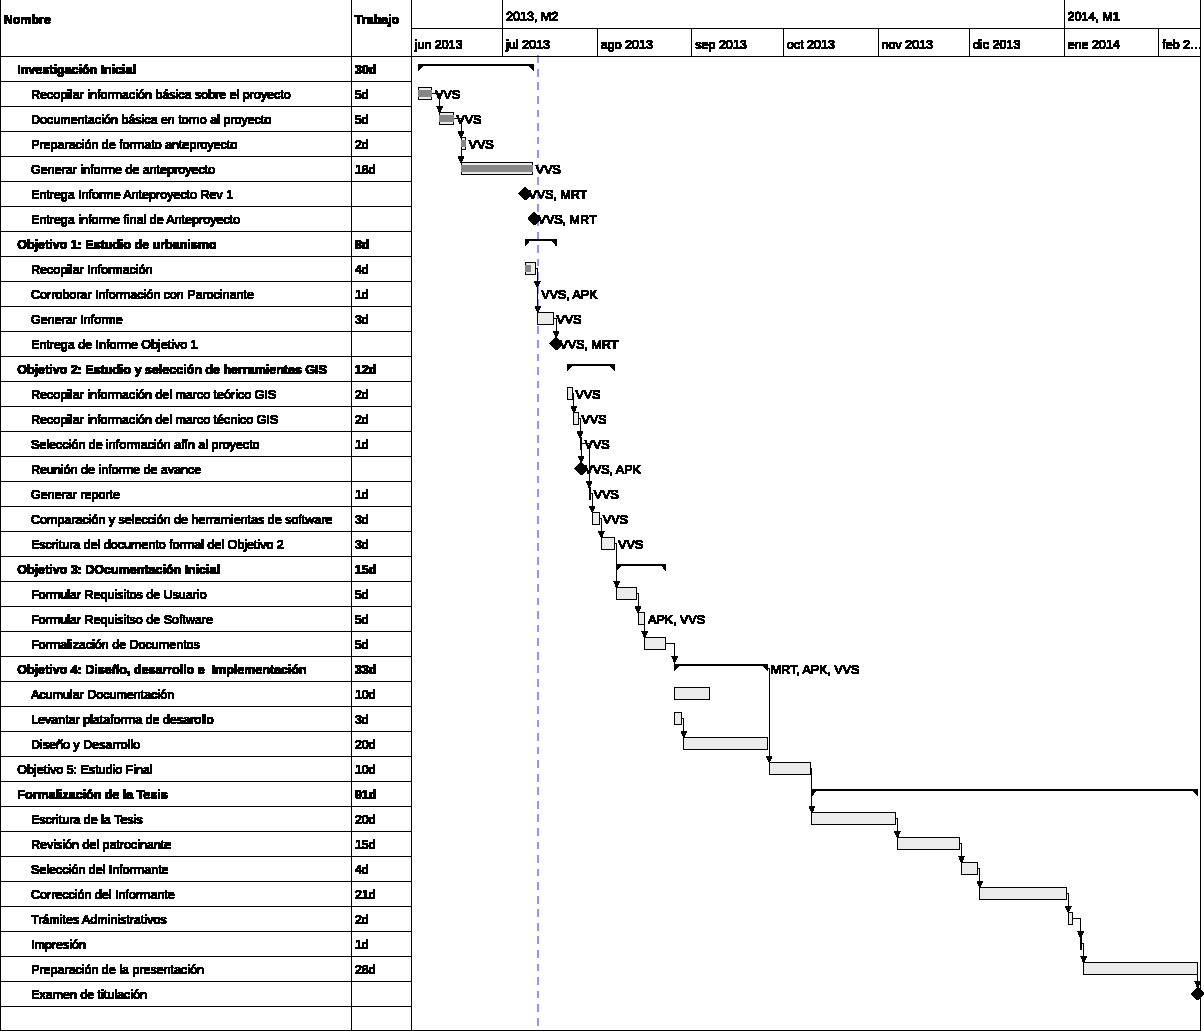
\includegraphics[scale=.9,angle=90]{imagenes/gantt.pdf}
\end{figure}

\begin{figure}[!hp]
    \caption{Descripción de las Tareas de la Carta Gantt}
    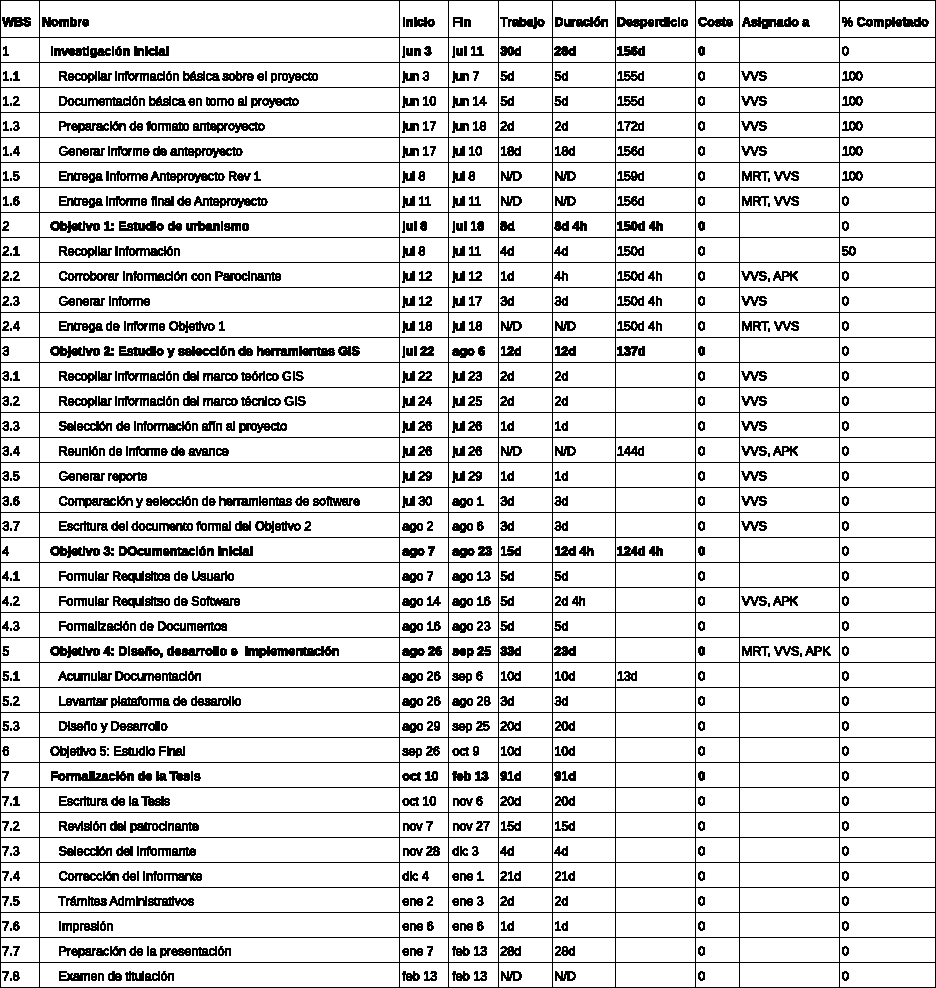
\includegraphics[scale=1]{imagenes/tareas.pdf}
\end{figure}

\newpage
\section{presupuesto del proyecto}
\begin{table}[h]
	\begin{tabular}{|l|l|l|l|}
    \cline{3-3}
    \multicolumn{1}{l}{} &  &\cellcolor{lightgray} \textbf{\sffamily Aporte de	Terceros} & \multicolumn{1}{l}{} \\ 
    \hline
    \rowcolor{tableheadcolor} \textbf{\sffamily Ítem} & \textbf{\sffamily
    Aporte Ejecutor} & \textbf{\sffamily SECPLAN} & \textbf{\sffamily TOTAL} \\ 
    \hline
    Incentivos y Honorarios & \$1.800.000 & -- & \$1.800.000 \\ 
    \hline
    Costos de Producción & \$1.254.000 & -- & \$1.254.000 \\ 
    \hline
    Pasajes y Viáticos & \$288.000 & -- & \$288.000  \\ 
    \hline
    Equipamiento & \$373.500 & -- & \$373.500 \\ 
    \hline
    Material Fungible & \$7.500 & \$42.000 & \$49.500 \\ 
    \hline
    Difusión & -- & \$30.000 & \$30.000 \\ 
    \hline
    Gastos Generales & \$46.500 & -- & \$46.500 \\ 
    \hline
    Actividad de Difusión & -- & -- & -- \\ 
    \hline
    \rowcolor{tableheadcolor} \textbf{\sffamily TOTAL} &\$3.769.500 & \$72.000 & \$3.841.500\\
    \hline
    \rowcolor{tableheadcolor} \textbf{\sffamily Porcentajes} &98\% &2\% &100\% \\
    \hline
	\end{tabular}
\end{table}

\subsection{justificación}

\begin{itemize}
    \item Incentivos y Honorarios: Corresponde a la suma total del sueldo
      asignado al análisis, diseño y desarrollo del proyecto, siendo de
      \$300.000 mensuales, sumando \$1.800.000 en el total del ejercicio
      aportado por el ejecutor.
    \item Costos de Producción: Considerando el arriendo de las oficinas a
      \$150.000 mensuales, \$27.000 mensuales en cobro de servicios de
      telefonía e Internet, \$11.000 mensual en cobro de electricidad y
      \$7.000 en gastos mensual; cada uno durante seis meses. Añadiendo los
      costos de calefacción durante tres meses que sumados corresponden a
      \$84.000 el total de el aporte del ejecutor al proyecto es de
      \$1.254.000.
    \item Pasajes y Viáticos: Considerando 6 viajes de locomoción colectiva por
      semana a un costo de \$500 por viaje, con el fin de asistir a reuniones
      con el patrocinante y para recaudar información, se suman \$72.000 al
      total del presupuesto aportado por el ejecutor. Además se consideran
      \$36.000 mensuales en costos de alimentación, también aportados por el
      ejecutor. El total considerado como aporte para el proyecto son de
      \$288.000 para los seis meses de duración del proyecto.
    \item Equipamiento: El arriendo del equipo para desarrollo tiene un costo de
      \$21.000 mensual. El arriendo del equipo para servidor de pruebas, que
      incluye computador de escritorio y router, considera un costo de
      \$41.250 al mes. Sumado esto durante el total del ejercicio da un valor
      de \$373.500 aportados por el ejecutor.
    \item Material Fungible: Se estiman \$7.000 mensuales en costos de tinta e
      impresión, lo que suma un total de \$42.000 durante el ejercicio,
      aportados por la \textsc{secplan}. El ejecutor estima un aporte de \$7.500 total en
      gasto en elementos de oficina. La suma de estos aportes es de \$49.500 para
      el total del ejercicio.
    \item Difusión: Se considerarán los costos en cuanto a hosting y dominio del
      blog del proyecto, aproximado a un valor total de \$30.000 durante todo
      el ejercicio aportados por la SECPLAN.
    \item Gastos Generales: Se considerará un pozo de emergencias ante cualquier
      imprevisto de un total de \$46.500 aportados por el ejecutor.
\end{itemize}
\newpage
\section{plan de difusión del proyecto}
\begin{itemize}
    \item El desarrollo del proyecto se difundirá a través de un blog, que
      se publicará una vez comenzada la etapa del ciclo de vida del
      proyecto, dónde se mostrará el estado de avance del mismo y los
      resultados durante su desarrollo.
    \item Difusión entre los usuarios que utilizarán el prototipo.
    \item Plan de capacitación para juntas de vecinos y equipos de
      postulación a proyectos de urbanismo.
\end{itemize}

\end{document}
